\documentclass[conference]{IEEEtran}
%\documentclass[sigconf]{acmart}
\makeatletter
\def\ps@headings{%
\def\@oddhead{\mbox{}\scriptsize\rightmark \hfil \thepage}%
\def\@evenhead{\scriptsize\thepage \hfil \leftmark\mbox{}}%
\def\@oddfoot{}%
\def\@evenfoot{}}
\makeatother
\pagestyle{empty}
\usepackage{url}
\usepackage{graphicx,subfigure}
\usepackage{epstopdf}
\usepackage{amsmath}
\usepackage{algorithm}
\usepackage{algpseudocode}
\usepackage{amsmath}
\usepackage{amssymb}
\usepackage{amsthm}
\usepackage{epsfig}
\newtheorem{theorem}{Theorem}
\renewcommand{\algorithmicrequire}{\textbf{Input:}} % Use Input in the format of Algorithm
\renewcommand{\algorithmicensure}{\textbf{Output:}} % Use Output in the format of Algorithm
\usepackage{amsfonts}
%\newtheorem{theorem}{Theorem}[section]
\newtheorem{mydef}{Definition}[section]
%\newtheorem{lemma}{Lemma}[section]
\usepackage{multirow}
\usepackage{color}
\usepackage{array}
\usepackage{listings}
\usepackage{hyperref}
\usepackage[underline=true]{pgf-umlsd}
\newcommand{\tabincell}[2]
{\begin{tabular}
		{@{}#1@{}}#2\end{tabular}}
\usepackage{setspace}
\renewcommand{\labelitemi}{$\vcenter{\hbox{\tiny$\bullet$}}$}


\hyphenation{op-tical net-works semi-conduc-tor}
\graphicspath{ {./images/} }



\begin{document}



\title{Replace with Your Project Title}

\author{\IEEEauthorblockN{1\textsuperscript{st} Given Name Surname}
\IEEEauthorblockA{\textit{dept. name of organization (of Aff.)} \\
\textit{name of organization (of Aff.)}\\
City, Country \\
email address}
\and
\IEEEauthorblockN{2\textsuperscript{nd} Given Name Surname}
\IEEEauthorblockA{\textit{dept. name of organization (of Aff.)} \\
\textit{name of organization (of Aff.)}\\
City, Country \\
email address}
\and
\IEEEauthorblockN{3\textsuperscript{rd} Given Name Surname}
\IEEEauthorblockA{\textit{dept. name of organization (of Aff.)} \\
\textit{name of organization (of Aff.)}\\
City, Country \\
email address}
}

\maketitle


\begin{abstract}
Phishing is an evident cybersecurity threat. Cybercriminals often pose as reputable organizations and send emails with links to phishing websites to unsuspecting individuals. Individuals who enter phishing websites, expose themselves to data breaches and malware. Companies spend time and money investing in cybersecurity training to protect their employees and customers from phishing attempts. Nevertheless, phishing is still prevalent in today’s society. In an October 2022 study, conducted by security provider SlashNext, found more than 255 million phishing attempts in email, mobile, and browser channels. SlashNext reports that there has been a 61% increase in phishing attempts since 2021. To solve this problem, we propose to create a phishing detection system based on machine learning algorithms. The problem is essentially a classification task of whether a link is legitimate or phishing. We will train the model to detect a phishing website based on a subset of features. 
\end{abstract}

\section{Introduction}
The section includes SEVERAL paragraphs summarizing your project. It is like the extended version of Abstract - you may use one paragraph for each of these parts - problem statement, dataset description, machine learning algorithms you will use to solve the problem, experimental results, and how your solutions are better as compared to existing solutions. Please try to limit Introduction to one page.

\section{Related Work}
This section summarizes existing solutions to the problem or similar problems. Please try to categorize these existing techniques and provide some discussion on the pros and cons of them. Don't forget to include references to any existing work you mention.  

\section{Our Solution}
This section elaborates your solution to the problem.

\subsection{Description of Dataset}
The features we are using from the dataset to train the model are the following: "https_token", "ratio_digits_url", "nb_hyphens", "nb_dots", "nb_underscore", "nb_slash". Some of these features are discrete (0 or 1) and some are continuous values. Features that hold discrete values help describe whether something is present or not in the URL (i.e hyphens), while continuous values quantify a feature of the URL (i.e ratio of digits).

\subsection{Machine Learning Algorithms}
One machine learning we will be using is KNN-classifier. The values "phishing" and "legitimate" will be encoded to 0 and 1, respectively. 

\subsection{Implementation Details}
The date is split into a training size of 75 percent, and a dataset for testing of size 25 percent of the entire dataset. To optimize this algorithm, we are collecting the best value of k 'best_k', which is shown in the graph below:
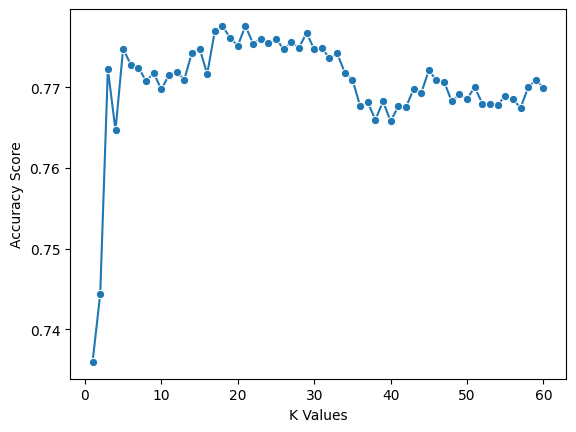
\includegraphics{best-k-value.png}

\section{Comparison}  
This section includes the following: 1) comparing the performance of different machine learning algorithms that you used, and 2) comparing the performance of your algorithms with existing solutions if any. Please provide insights to reason about why this algorithm is better/worse than another one.

\section{Future Directions}
This section lays out some potential directions for further improving the performance. You can image what you may do if you were given extra 3-6 months.

\section{Conclusion}
This section summarizes this project, i.e., by the extensive experiments and analysis, do you think the problem is solved well? which algorithm(s) might be better suitable for this problem? Which technique(s) may help further improve the performance? \\

Last but not the least, don't forget to include references to any work you mentioned in the report.
  

\bibliographystyle{IEEEtran}
\bibliography{}


\end{document}


